\documentclass[letterpaper,12pt]{report}
\usepackage[margin=1in]{geometry}
\usepackage{fancyhdr,tocloft,url,graphicx,float,listings,sidecap,wrapfig}
\usepackage[numbers]{natbib}
\usepackage[font=small,labelfont=bf,labelsep=period]{caption}
\usepackage{tabularx}
\usepackage{setspace}
% \usepackage{hyperref}
% \usepackage[all]{hypcap}
\usepackage{qtree,algorithm,algorithmic}
\usepackage{tcolorbox}
\usepackage{textcomp}
\usepackage{enumitem}
\usepackage{xcolor}
\usepackage{tikz}
\usepackage{times}
\usepackage[utf8]{inputenc}

\pagestyle{plain}
\fancyhf{}
\lhead{}
\chead{}
\rhead{}
\cfoot{\thepage}


%\floatstyle{boxed}
%\restylefloat{figure}

% \hypersetup {
% 	colorlinks=false,
% 	pdfborder={0 0 0},
% }

\setcounter{secnumdepth}{3}
\renewcommand*\thesection{\arabic{section}.}
\renewcommand*\thesubsection{\thesection\arabic{subsection}.}
\renewcommand*\thesubsubsection{\thesubsection\arabic{subsubsection}.}

\setcounter{tocdepth}{3}
\renewcommand\contentsname{}				% TOC title
\renewcommand\listfigurename{}				% LOF title
\renewcommand\listtablename{}				% LOT title
\setlength\cftaftertoctitleskip{-0.5in}
\setlength\cftafterloftitleskip{-0.5in}
\setlength\cftafterlottitleskip{-0.5in}
\makeatletter
\def\blfootnote{\xdef\@thefnmark{}\@footnotetext}
\makeatother

\newcommand*\circled[1]{\tikz[baseline=(char.base)]{
            \node[shape=circle,fill=black,inner sep=1pt] (char) {\textcolor{white}{\small\bfseries #1}};}}

            \lstset{
                basicstyle=\ttfamily,
                breakindent=2em,
            }

\begin{document}

% \hypersetup{pageanchor=true}
%%  COVER PAGE
\begin{titlepage}
	\begin{center}
		\vspace*{0.5in}
		\begin{doublespace}
			\LARGE \textbf{\(P = NP\)} \\
			\vspace*{1in}
			\normalsize
			A Manuscript \\
			Submitted to \\
			the Department of Computer Science \\
			and the Faculty of the\\
			University of Wisconsin--La Crosse \\
			La Crosse, Wisconsin \\
			\vspace*{0.5in}
			by \\
			\large
			\textbf{Daniel Weninger} \\

			\vspace*{0.5in}
			\normalsize
			in Partial Fulfillment of the \\
			Requirements for the Degree of\\
			\Large{\textbf{Master of Software Engineering}} \\
			\normalsize
			May, 2023
		\end{doublespace}
	\end{center}
\end{titlepage}
	
\clearpage

%% SIGNATURE PAGE
\thispagestyle{empty}
\vspace*{0.3in}
\begin{center}
	\large{\textbf{\(P = NP\)}} \\ 
	\vspace{0.75in}
	\normalsize{By Johnny Q.\ Student}
\end{center}

\vspace{0.5in}
\noindent We recommend acceptance of this manuscript in partial fulfillment of this candidate's requirements for the degree of Master of Software Engineering in Computer Science. The candidate has completed the oral examination requirement of the capstone project for the degree. \\

\noindent
\begin{tabularx}{\textwidth}{p{3in}Xp{2in}}
	\rule{0pt}{50pt} & & \\
	\hrulefill & & \hrulefill \\
	Prof.\ Albert Einstein & & Date \\
	Examination Committee Chairperson & & \\
	\rule{0pt}{50pt} & & \\
	\hrulefill & & \hrulefill \\
	Prof.\ Isaac Newton & & Date \\
	Examination Committee Member & & \\
	\rule{0pt}{50pt} & & \\
	\hrulefill & & \hrulefill \\
	Prof.\ Marie Curie & & Date \\
	Examination Committee Member & & \\
\end{tabularx}


\clearpage

% \hypersetup{pageanchor=true}
\setcounter{page}{1}
\pagenumbering{roman}
\renewcommand\arraystretch{1.5}

%% ABSTRACT
\vspace*{0.5in}
\section*{Abstract}
\addcontentsline{toc}{section}{Abstract}
Weninger, Daniel, ``PAMEx: A Compiler and Tools to Support a 
More Flexible Security Policy for Simpleflow'' Master of Software 
Engineering, May 2023, (W. Michael Petullo, Ph.D.). \\

This manuscript describes the design and implementation of PAMEx, a custom-built Linux security tool 
suite that uses several aspects of modern Linux security modules to enforce its policies. 
The tool suite uses extended attributes to define file security information, a custom Pluggable Authentication Module (PAM) 
to define actions that occur when a user authenticates on a system, 
and a custom compiler developed with Flex and Bison. PAMEx was developed as a security enhancement for SimpleFlow, 
a project that uses information flows to enforce policies. The way that PAMEx provides this enhancement to SimpleFlow 
is by being able to classify and compartmentalize file security as hierarchical levels, and non-hierarchical labels 
rather than the binary policy that SimpleFlow currently has in place. 
As a simulation, a tool was created and given the name Oracle that, when queried, 
will output a response as to if a user has access to a particular file. This paper gives an overview of the design and 
implementation choices made during the development of PAMEx and future work that could be done to maintain and improve the project. 
\clearpage

%%% ACKNOWLEDGEMENTS
\vspace*{0.5in}
\section*{Acknowledgements}
\addcontentsline{toc}{section}{Acknowledgments}
\par 
\hspace{1em}
I would like to give my sincerest gratitude and thanks to my advisor, Dr. Petullo. Without whom I would not have been able to get as far as I had or learn as much as I did during the development of my capstone project.
\clearpage

%% TABLE OF CONTENTS
\vspace*{0.5in}
\section*{Table of Contents}
\tableofcontents
\clearpage


% %% LIST OF TABLES
% \section*{List of Tables}
% \addcontentsline{toc}{section}{List of Tables}
% \listoftables
% \clearpage

%% LIST OF FIGURES
\vspace*{0.5in}
\section*{List of Figures}
\addcontentsline{toc}{section}{List of Figures}
\listoffigures
\clearpage

%% GLOSSARY
\vspace*{0.5in}
\section*{Glossary}
\addcontentsline{toc}{section}{Glossary}
\subsubsection*{Agile}

A project management philosophy which uses an iterative approach. Each iteration is a working product whose next iteration semantics can be changed \cite{kung2014}.

\subsubsection*{Bison}

A parser that translates a BNF grammar from the tokens that a lexical analyzer makes into groupings of statements. The statements determine which functions to perform \cite{levine2009}.

\subsubsection*{Extended Attributes}

Key-value paired metadata attached to files. Extended attributes are written to in PAMEx to store the security level and labels attached to the file. 

\subsubsection*{Flex}

The program used in PAMEx to create a lexical analyzer or scanner. Flex creates a character stream from defined, recognizable tokens and therefore outlines legal words that can be used in a system \cite{levine2009}.

\subsubsection*{Label}

A non-hierarchical compartment defined by the privileged administrative user. A file can have zero or more labels in addition to a level to further define its security. For a user to access a file with PAMEx security labels, the user must have the same corresponding labels. 

\subsubsection*{Level}

A hierarchical compartment defined by the privileged administrative user. Each level in a PAMEx system has its own placement and each file on a system can be assigned a level. To access a file with a PAMEx level, a user must be assigned a level whose placement is equivalent to the file’s level or higher.

\subsubsection*{Linux Security Module}

A framewok integrated into the Linux kernel which provides access controls to processes, files, and other aspects of the Linux system \cite{kerneldocs}.

\subsubsection*{PAMEx}

The Linux security tool suite developed to enhance the SimpleFlow project. 

\subsubsection*{Level Placement}

The hierarchical value of a level in PAMEx. Placements start at level zero for unrestricted access to a file and relationally go up by one. No two levels on the same system can share a placement value. 

\subsubsection*{Pluggable Authentication Module (PAM)}

A separated process or task which is invoked during the authentication process. PAM modules are stacked to be invoked consecutively \cite{lauber}.

\subsubsection*{Scrum}

A framework for the Agile method which uses a cyclical approach called a sprint. The sprint team consists of a scrum master, one or more product owners, and developers. Scrum outlines actions that occur to achieve an iterative product at the end of each sprint \cite{scrumorg}.

\subsubsection*{Sprint}

One cycle in the Scrum process. The PAMEx sprint time was two weeks.

\subsubsection*{sudo-proc}
The fake process file directory that PAMEx's PAM module creates. PAMEx creates this directory because it does not have privileges to write to actual process files on the system.


\clearpage

\setcounter{page}{1}
\pagenumbering{arabic}

\IfFileExists{section01/section}{\section{Introduction}
\newcounter{numitem}

\label{sec:Introduction}
\vspace{\baselineskip}

\subsection{Background}
\par 
\vspace{\baselineskip}
\hspace{1em}
The objective of PAMEx is to work in conjunction with and enhance the 
pre-existing project SimpleFlow, an information-flow-based access 
control system. Even in the modern day, most access control systems 
simply disallow read or write access to confidential files. The 
SimpleFlow project was developed to go beyond most access control 
systems and instead allow malicious users to access confidential 
files up until the point of exfiltration so that SimpleFlow can monitor the user's activity. The way that 
SimpleFlow achieves this is by working on top of the Linux Security 
Module (LSM) interface and rather than simply disallowing read or write 
access like most access control systems do, SimpleFlow instead marks a 
file as either confidential or non-confidential. If a confidential 
file is wrongly accessed, the malicious user’s actions are recorded as they pass 
through the system as information flows. The wrongly accessed 
information is then prevented from being exfiltrated by SimpleFlow's network filter. 
SimpleFlow begins tracking the attacker’s actions as soon as they 
attempt to access the confidential file and therefore can capture the attacker’s 
intentions. This leaves no room for the malicious user to come up with 
a fabricated excuse as to why they were trying to exfiltrate sensitive 
information. As an example of SimpleFlow’s effectiveness, when put to 
practical use during the 2016 Cyber-Defense Exercise, the SimpleFlow 
program proved to perform well with a small overhead. While the 
practical exercise did not make use of all SimpleFlow’s functionality, 
it was able to successfully use SimpleFlow’s network filter which made 
it easy to observe any attempt at exfiltrating data. Within this 
exercise and other testing, SimpleFlow impressed attackers who were 
surprised to find their exfiltration attempts had failed \cite{ryan2016}. 

Figure~\ref{simpleflowexample} was pulled from the paper ``Studying Naive Users and the Insider Threat with SimpleFlow.''
to depict SimpleFlow being used to prevent an exfiltration attempt of sensitive data.
The example starts with a file on the kernel marked as \texttt{secret} which contains sensitive information.

\clearpage

\begin{figure}[h]
    \centering
    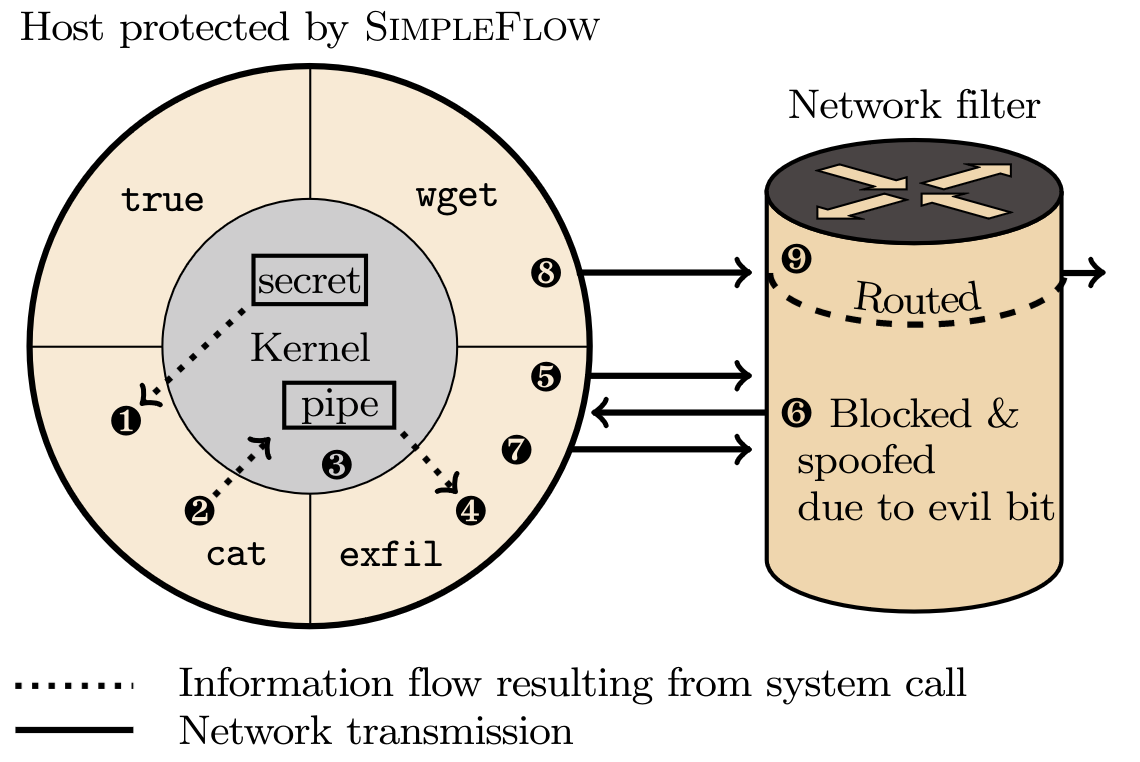
\includegraphics[width=.8\textwidth]{section01/assets/simpleflow_example.png}
    \caption[SimpleFlow Example]{SimpleFlow Being Used to Prevent Exfiltration of Sensitive Data (from \cite{ryan2016})\label{simpleflowexample}}
\end{figure}
\blfootnote{The above numerical SimpleFlow example items were summarized from \cite{ryan2016}.}
\begin{enumerate}[label={\protect\circled{\arabic*}}]
    \item A malicious user uses the \texttt{cat} process to open and read the confidential data in \texttt{secret}.
          Now any further actions processed by this user are tainted by SimpleFlow by being marked with an evil bit 
          and are monitored by the SimpleFlow system.
    \item The malicious user attempts to pipe and exfiltrate the information in \texttt{secret}.
    \item The pipe is forked as a child from the \texttt{cat} process and therefore is also marked as malicious activity by SimpleFlow.
    \item The \texttt{exfil} command reads \texttt{secret} and becomes tainted with the evil bit.
    \item The malicious user attepts to exfiltrate the information from \texttt{secret} to a personal server. 
          The sent packet containing \texttt{secret}'s
          information is marked with an evil bit to be easily recognizable by SimpleFlow as an unsolicited action.
    \item SimpleFlow's network filter notices the malicious user's attempt to exfiltrate the information from \texttt{secret}.
          SimpleFlow sends a fake response to the request to make the malicious user think that the process is being continued.
    \item The malicious user's exfiltration attept on \texttt{secret}'s data is ultimately blocked by SimpleFlow's network filter.
    \item The non-threatening process \texttt{wget} is performed on the system.
    \item SimpleFlow's network filter behaves normally and allows the \texttt{wget} process to continue.
\end{enumerate}


While effective, the research prototype of SimpleFlow is limited in 
that it cannot further specify the security policy of a file beyond 
being confidential and non-confidential \cite{ryan2016}. A resolution 
for SimpleFlow’s issue of a binary security system was therefore sought out and as a solution 
a customized Linux security tool suite was devised. The system would allow the 
privileged user to define hierarchical levels and non-hierarchical 
labels on a system and assign them to both system users and system 
files. This security policy was inspired by the US security 
classification system \cite{natsecinfo} by following the structure of having both levels 
and labels for security. The policy states that both system files and system users may each have one 
security level and zero or more security labels. 

As a running example, pretend that
there is a software company that is working on innovative technology that they want
to be kept secretive so that all files related to the technology are on a need-to-know basis. 
With this proposed security policy, the company could define a system saying which staff have
access to what files. For example, the privileged administrative user who oversees creating the security policy 
could define the hierarchy levels for the company from lowest to highest as
\texttt{public}, \texttt{general\_staff}, \texttt{developer}, \texttt{administrator}, and \texttt{executive\_staff}.
In this example, the company has also split the technology into several projects, 
three of which are named \texttt{alpha}, \texttt{beta}, and \texttt{charlie}. If Alice is an \texttt{administrator} for
both projects \texttt{alpha} and \texttt{beta}, then, with the newly proposed security policy,
she would be given the hierarchical level \texttt{administrator} and the non-hierarchical labels
\texttt{alpha} and \texttt{beta}. 

Continuing the above example, pretend that there is a file to outline how to begin development on project \texttt{alpha} called
\texttt{alpha}\texttt{\_dev}\texttt{\_instructions.txt}. The privileged administrator could assign \texttt{alpha}\texttt{\_dev}\texttt{\_instructions.txt} 
the security level \texttt{developer} and the security label \texttt{alpha}. Alice, who has the security level of \texttt{administrator}
which is placed higher than \texttt{developer} in the level hierarchy 
and who contains the security label \texttt{alpha} can access \texttt{alpha}\texttt{\_dev}\texttt{\_instructions.txt}.
Pretend that there is also a developer in the company named Bob who is a developer for projects \texttt{beta} and \texttt{charlie}. Bob would
have the security level \texttt{developer} which is a proper label to be able to access \texttt{alpha}\texttt{\_dev}\texttt{\_instructions.txt}, but Bob would not
be given the label \texttt{alpha} so therefore would ultimately not have access to \texttt{alpha}\texttt{\_dev}\texttt{\_instructions.txt}.

The newly proposed security policy of levels and labels 
would allow multiple groupings of users such as, in our example, 
more \texttt{developer}s who have access to project \texttt{alpha}, more \texttt{administrator}s that 
have access to multiple projects,
and files that are available to all staff members. With the newly proposed security policy, 
a system administrator would therefore be able 
to flexibly compartmentalize all the files and data that users would have 
access to on a system. Initially, it may seem like other previously-developed access control models may be sufficient
to create a security policy that is ideal for SimpleFlow such as role-based access controls (RBAC).
However, these models are not as ideal as the newly proposed PAMEx secuirty policy.
As stated above, most RBAC simply disallow reading or writing to confidential files on a system, but SimpleFlow 
wants to instead allow that access so as to be able to monitor an attacker's actions. SimpleFlow's primary job is
to record a malicious user's activity on the system and ultimately disallow exfiltrating confidential information
via its network filter. With SimpleFlow having such a particular goal, only a custom security policy such as PAMEx will allow SimpleFlow
to continue to monitor a system the way that it was designed to without interfering with SimpleFlow's actions.
Ideally, the tool suite would be developed as a standalone 
Linux Security Module so as to be tailored to but not mutually 
exclusive for SimpleFlow though. The development of the custom kernel module that would allow the tool suite to be standalone
or ported into SimpleFlow was left to future work.


\subsection{Motivation}
\par 
\vspace{\baselineskip}
\hspace{1em}
In 2022, the author reached out to his advisor, Dr. W. Michael 
Petullo showing interest in the SimpleFlow project and learning more about 
its shortcomings including the binary security policy currently in 
place. Having pursued an emphasis in cybersecurity alongside his 
degree, the author had already had an introduction to Linux security 
but wanted to learn more. The motivation of PAMEx was to aid in and 
further enhance the development of the SimpleFlow project as well as 
to learn more about Linux security at a system level and how it can 
be added to and manipulated. Building a security policy tool system 
from the ground up would give a foundational experience of 
that aspect of security systems. 

Together with his advisor, the author devised and proposed an 
alternative solution for the SimpleFlow security policy than the 
one currently in place. This policy would continue to work on top 
of the LSM interface as SimpleFlow already does and therefore be 
integrated into SimpleFlow easily. The policy’s syntax and 
tools would be user friendly and allow for much greater malleability 
while having a small footprint. Another requirement was to ensure 
that PAMEx's integration would not need to be exclusive 
to SimpleFlow but could be used on many Linux based systems. Developing 
a project of this scale is also a perfect opportunity to research, learn about, and practice the development cycle of 
a project with industry standards.  

}{}\clearpage
\IfFileExists{section03/section}{\section{Introduction}
\newcounter{numitem}

\label{sec:Introduction}
\vspace{\baselineskip}

\subsection{Background}
\par 
\vspace{\baselineskip}
\hspace{1em}
The objective of PAMEx is to work in conjunction with and enhance the 
pre-existing project SimpleFlow, an information-flow-based access 
control system. Even in the modern day, most access control systems 
simply disallow read or write access to confidential files. The 
SimpleFlow project was developed to go beyond most access control 
systems and instead allow malicious users to access confidential 
files up until the point of exfiltration so that SimpleFlow can monitor the user's activity. The way that 
SimpleFlow achieves this is by working on top of the Linux Security 
Module (LSM) interface and rather than simply disallowing read or write 
access like most access control systems do, SimpleFlow instead marks a 
file as either confidential or non-confidential. If a confidential 
file is wrongly accessed, the malicious user’s actions are recorded as they pass 
through the system as information flows. The wrongly accessed 
information is then prevented from being exfiltrated by SimpleFlow's network filter. 
SimpleFlow begins tracking the attacker’s actions as soon as they 
attempt to access the confidential file and therefore can capture the attacker’s 
intentions. This leaves no room for the malicious user to come up with 
a fabricated excuse as to why they were trying to exfiltrate sensitive 
information. As an example of SimpleFlow’s effectiveness, when put to 
practical use during the 2016 Cyber-Defense Exercise, the SimpleFlow 
program proved to perform well with a small overhead. While the 
practical exercise did not make use of all SimpleFlow’s functionality, 
it was able to successfully use SimpleFlow’s network filter which made 
it easy to observe any attempt at exfiltrating data. Within this 
exercise and other testing, SimpleFlow impressed attackers who were 
surprised to find their exfiltration attempts had failed \cite{ryan2016}. 

Figure~\ref{simpleflowexample} was pulled from the paper ``Studying Naive Users and the Insider Threat with SimpleFlow.''
to depict SimpleFlow being used to prevent an exfiltration attempt of sensitive data.
The example starts with a file on the kernel marked as \texttt{secret} which contains sensitive information.

\clearpage

\begin{figure}[h]
    \centering
    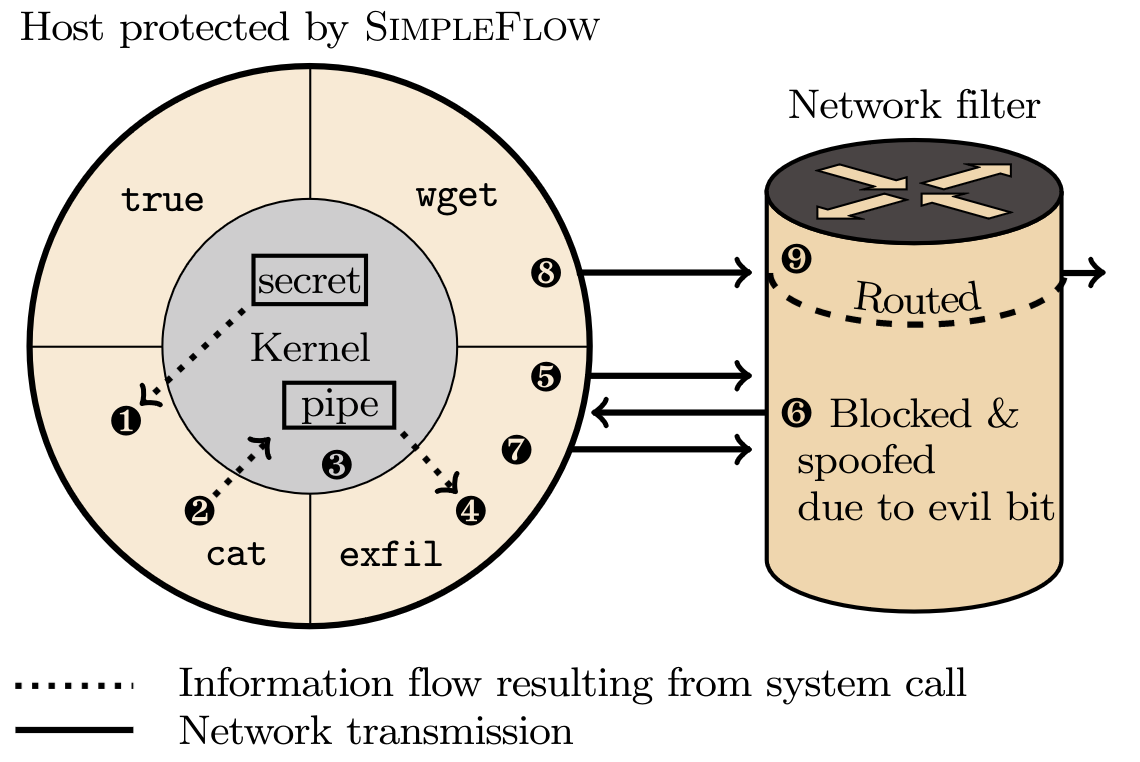
\includegraphics[width=.8\textwidth]{section01/assets/simpleflow_example.png}
    \caption[SimpleFlow Example]{SimpleFlow Being Used to Prevent Exfiltration of Sensitive Data (from \cite{ryan2016})\label{simpleflowexample}}
\end{figure}
\blfootnote{The above numerical SimpleFlow example items were summarized from \cite{ryan2016}.}
\begin{enumerate}[label={\protect\circled{\arabic*}}]
    \item A malicious user uses the \texttt{cat} process to open and read the confidential data in \texttt{secret}.
          Now any further actions processed by this user are tainted by SimpleFlow by being marked with an evil bit 
          and are monitored by the SimpleFlow system.
    \item The malicious user attempts to pipe and exfiltrate the information in \texttt{secret}.
    \item The pipe is forked as a child from the \texttt{cat} process and therefore is also marked as malicious activity by SimpleFlow.
    \item The \texttt{exfil} command reads \texttt{secret} and becomes tainted with the evil bit.
    \item The malicious user attepts to exfiltrate the information from \texttt{secret} to a personal server. 
          The sent packet containing \texttt{secret}'s
          information is marked with an evil bit to be easily recognizable by SimpleFlow as an unsolicited action.
    \item SimpleFlow's network filter notices the malicious user's attempt to exfiltrate the information from \texttt{secret}.
          SimpleFlow sends a fake response to the request to make the malicious user think that the process is being continued.
    \item The malicious user's exfiltration attept on \texttt{secret}'s data is ultimately blocked by SimpleFlow's network filter.
    \item The non-threatening process \texttt{wget} is performed on the system.
    \item SimpleFlow's network filter behaves normally and allows the \texttt{wget} process to continue.
\end{enumerate}


While effective, the research prototype of SimpleFlow is limited in 
that it cannot further specify the security policy of a file beyond 
being confidential and non-confidential \cite{ryan2016}. A resolution 
for SimpleFlow’s issue of a binary security system was therefore sought out and as a solution 
a customized Linux security tool suite was devised. The system would allow the 
privileged user to define hierarchical levels and non-hierarchical 
labels on a system and assign them to both system users and system 
files. This security policy was inspired by the US security 
classification system \cite{natsecinfo} by following the structure of having both levels 
and labels for security. The policy states that both system files and system users may each have one 
security level and zero or more security labels. 

As a running example, pretend that
there is a software company that is working on innovative technology that they want
to be kept secretive so that all files related to the technology are on a need-to-know basis. 
With this proposed security policy, the company could define a system saying which staff have
access to what files. For example, the privileged administrative user who oversees creating the security policy 
could define the hierarchy levels for the company from lowest to highest as
\texttt{public}, \texttt{general\_staff}, \texttt{developer}, \texttt{administrator}, and \texttt{executive\_staff}.
In this example, the company has also split the technology into several projects, 
three of which are named \texttt{alpha}, \texttt{beta}, and \texttt{charlie}. If Alice is an \texttt{administrator} for
both projects \texttt{alpha} and \texttt{beta}, then, with the newly proposed security policy,
she would be given the hierarchical level \texttt{administrator} and the non-hierarchical labels
\texttt{alpha} and \texttt{beta}. 

Continuing the above example, pretend that there is a file to outline how to begin development on project \texttt{alpha} called
\texttt{alpha}\texttt{\_dev}\texttt{\_instructions.txt}. The privileged administrator could assign \texttt{alpha}\texttt{\_dev}\texttt{\_instructions.txt} 
the security level \texttt{developer} and the security label \texttt{alpha}. Alice, who has the security level of \texttt{administrator}
which is placed higher than \texttt{developer} in the level hierarchy 
and who contains the security label \texttt{alpha} can access \texttt{alpha}\texttt{\_dev}\texttt{\_instructions.txt}.
Pretend that there is also a developer in the company named Bob who is a developer for projects \texttt{beta} and \texttt{charlie}. Bob would
have the security level \texttt{developer} which is a proper label to be able to access \texttt{alpha}\texttt{\_dev}\texttt{\_instructions.txt}, but Bob would not
be given the label \texttt{alpha} so therefore would ultimately not have access to \texttt{alpha}\texttt{\_dev}\texttt{\_instructions.txt}.

The newly proposed security policy of levels and labels 
would allow multiple groupings of users such as, in our example, 
more \texttt{developer}s who have access to project \texttt{alpha}, more \texttt{administrator}s that 
have access to multiple projects,
and files that are available to all staff members. With the newly proposed security policy, 
a system administrator would therefore be able 
to flexibly compartmentalize all the files and data that users would have 
access to on a system. Initially, it may seem like other previously-developed access control models may be sufficient
to create a security policy that is ideal for SimpleFlow such as role-based access controls (RBAC).
However, these models are not as ideal as the newly proposed PAMEx secuirty policy.
As stated above, most RBAC simply disallow reading or writing to confidential files on a system, but SimpleFlow 
wants to instead allow that access so as to be able to monitor an attacker's actions. SimpleFlow's primary job is
to record a malicious user's activity on the system and ultimately disallow exfiltrating confidential information
via its network filter. With SimpleFlow having such a particular goal, only a custom security policy such as PAMEx will allow SimpleFlow
to continue to monitor a system the way that it was designed to without interfering with SimpleFlow's actions.
Ideally, the tool suite would be developed as a standalone 
Linux Security Module so as to be tailored to but not mutually 
exclusive for SimpleFlow though. The development of the custom kernel module that would allow the tool suite to be standalone
or ported into SimpleFlow was left to future work.


\subsection{Motivation}
\par 
\vspace{\baselineskip}
\hspace{1em}
In 2022, the author reached out to his advisor, Dr. W. Michael 
Petullo showing interest in the SimpleFlow project and learning more about 
its shortcomings including the binary security policy currently in 
place. Having pursued an emphasis in cybersecurity alongside his 
degree, the author had already had an introduction to Linux security 
but wanted to learn more. The motivation of PAMEx was to aid in and 
further enhance the development of the SimpleFlow project as well as 
to learn more about Linux security at a system level and how it can 
be added to and manipulated. Building a security policy tool system 
from the ground up would give a foundational experience of 
that aspect of security systems. 

Together with his advisor, the author devised and proposed an 
alternative solution for the SimpleFlow security policy than the 
one currently in place. This policy would continue to work on top 
of the LSM interface as SimpleFlow already does and therefore be 
integrated into SimpleFlow easily. The policy’s syntax and 
tools would be user friendly and allow for much greater malleability 
while having a small footprint. Another requirement was to ensure 
that PAMEx's integration would not need to be exclusive 
to SimpleFlow but could be used on many Linux based systems. Developing 
a project of this scale is also a perfect opportunity to research, learn about, and practice the development cycle of 
a project with industry standards.  

}{}\clearpage
\IfFileExists{section04/section}{\section{Introduction}
\newcounter{numitem}

\label{sec:Introduction}
\vspace{\baselineskip}

\subsection{Background}
\par 
\vspace{\baselineskip}
\hspace{1em}
The objective of PAMEx is to work in conjunction with and enhance the 
pre-existing project SimpleFlow, an information-flow-based access 
control system. Even in the modern day, most access control systems 
simply disallow read or write access to confidential files. The 
SimpleFlow project was developed to go beyond most access control 
systems and instead allow malicious users to access confidential 
files up until the point of exfiltration so that SimpleFlow can monitor the user's activity. The way that 
SimpleFlow achieves this is by working on top of the Linux Security 
Module (LSM) interface and rather than simply disallowing read or write 
access like most access control systems do, SimpleFlow instead marks a 
file as either confidential or non-confidential. If a confidential 
file is wrongly accessed, the malicious user’s actions are recorded as they pass 
through the system as information flows. The wrongly accessed 
information is then prevented from being exfiltrated by SimpleFlow's network filter. 
SimpleFlow begins tracking the attacker’s actions as soon as they 
attempt to access the confidential file and therefore can capture the attacker’s 
intentions. This leaves no room for the malicious user to come up with 
a fabricated excuse as to why they were trying to exfiltrate sensitive 
information. As an example of SimpleFlow’s effectiveness, when put to 
practical use during the 2016 Cyber-Defense Exercise, the SimpleFlow 
program proved to perform well with a small overhead. While the 
practical exercise did not make use of all SimpleFlow’s functionality, 
it was able to successfully use SimpleFlow’s network filter which made 
it easy to observe any attempt at exfiltrating data. Within this 
exercise and other testing, SimpleFlow impressed attackers who were 
surprised to find their exfiltration attempts had failed \cite{ryan2016}. 

Figure~\ref{simpleflowexample} was pulled from the paper ``Studying Naive Users and the Insider Threat with SimpleFlow.''
to depict SimpleFlow being used to prevent an exfiltration attempt of sensitive data.
The example starts with a file on the kernel marked as \texttt{secret} which contains sensitive information.

\clearpage

\begin{figure}[h]
    \centering
    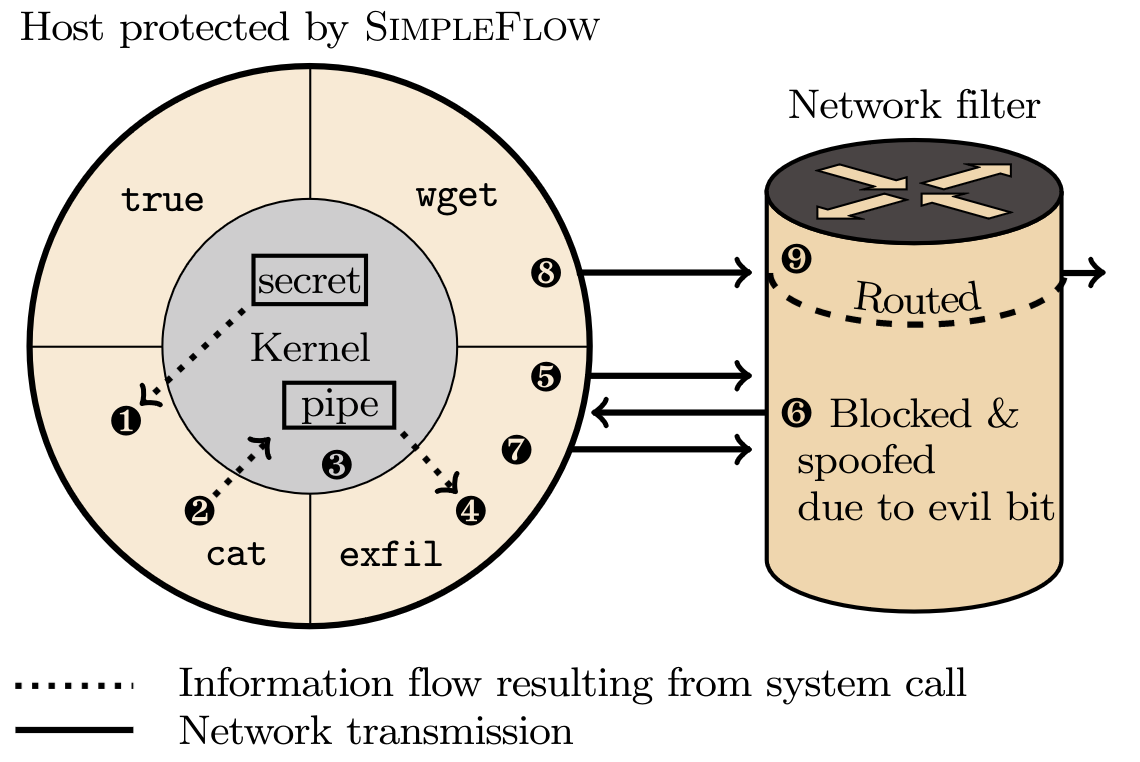
\includegraphics[width=.8\textwidth]{section01/assets/simpleflow_example.png}
    \caption[SimpleFlow Example]{SimpleFlow Being Used to Prevent Exfiltration of Sensitive Data (from \cite{ryan2016})\label{simpleflowexample}}
\end{figure}
\blfootnote{The above numerical SimpleFlow example items were summarized from \cite{ryan2016}.}
\begin{enumerate}[label={\protect\circled{\arabic*}}]
    \item A malicious user uses the \texttt{cat} process to open and read the confidential data in \texttt{secret}.
          Now any further actions processed by this user are tainted by SimpleFlow by being marked with an evil bit 
          and are monitored by the SimpleFlow system.
    \item The malicious user attempts to pipe and exfiltrate the information in \texttt{secret}.
    \item The pipe is forked as a child from the \texttt{cat} process and therefore is also marked as malicious activity by SimpleFlow.
    \item The \texttt{exfil} command reads \texttt{secret} and becomes tainted with the evil bit.
    \item The malicious user attepts to exfiltrate the information from \texttt{secret} to a personal server. 
          The sent packet containing \texttt{secret}'s
          information is marked with an evil bit to be easily recognizable by SimpleFlow as an unsolicited action.
    \item SimpleFlow's network filter notices the malicious user's attempt to exfiltrate the information from \texttt{secret}.
          SimpleFlow sends a fake response to the request to make the malicious user think that the process is being continued.
    \item The malicious user's exfiltration attept on \texttt{secret}'s data is ultimately blocked by SimpleFlow's network filter.
    \item The non-threatening process \texttt{wget} is performed on the system.
    \item SimpleFlow's network filter behaves normally and allows the \texttt{wget} process to continue.
\end{enumerate}


While effective, the research prototype of SimpleFlow is limited in 
that it cannot further specify the security policy of a file beyond 
being confidential and non-confidential \cite{ryan2016}. A resolution 
for SimpleFlow’s issue of a binary security system was therefore sought out and as a solution 
a customized Linux security tool suite was devised. The system would allow the 
privileged user to define hierarchical levels and non-hierarchical 
labels on a system and assign them to both system users and system 
files. This security policy was inspired by the US security 
classification system \cite{natsecinfo} by following the structure of having both levels 
and labels for security. The policy states that both system files and system users may each have one 
security level and zero or more security labels. 

As a running example, pretend that
there is a software company that is working on innovative technology that they want
to be kept secretive so that all files related to the technology are on a need-to-know basis. 
With this proposed security policy, the company could define a system saying which staff have
access to what files. For example, the privileged administrative user who oversees creating the security policy 
could define the hierarchy levels for the company from lowest to highest as
\texttt{public}, \texttt{general\_staff}, \texttt{developer}, \texttt{administrator}, and \texttt{executive\_staff}.
In this example, the company has also split the technology into several projects, 
three of which are named \texttt{alpha}, \texttt{beta}, and \texttt{charlie}. If Alice is an \texttt{administrator} for
both projects \texttt{alpha} and \texttt{beta}, then, with the newly proposed security policy,
she would be given the hierarchical level \texttt{administrator} and the non-hierarchical labels
\texttt{alpha} and \texttt{beta}. 

Continuing the above example, pretend that there is a file to outline how to begin development on project \texttt{alpha} called
\texttt{alpha}\texttt{\_dev}\texttt{\_instructions.txt}. The privileged administrator could assign \texttt{alpha}\texttt{\_dev}\texttt{\_instructions.txt} 
the security level \texttt{developer} and the security label \texttt{alpha}. Alice, who has the security level of \texttt{administrator}
which is placed higher than \texttt{developer} in the level hierarchy 
and who contains the security label \texttt{alpha} can access \texttt{alpha}\texttt{\_dev}\texttt{\_instructions.txt}.
Pretend that there is also a developer in the company named Bob who is a developer for projects \texttt{beta} and \texttt{charlie}. Bob would
have the security level \texttt{developer} which is a proper label to be able to access \texttt{alpha}\texttt{\_dev}\texttt{\_instructions.txt}, but Bob would not
be given the label \texttt{alpha} so therefore would ultimately not have access to \texttt{alpha}\texttt{\_dev}\texttt{\_instructions.txt}.

The newly proposed security policy of levels and labels 
would allow multiple groupings of users such as, in our example, 
more \texttt{developer}s who have access to project \texttt{alpha}, more \texttt{administrator}s that 
have access to multiple projects,
and files that are available to all staff members. With the newly proposed security policy, 
a system administrator would therefore be able 
to flexibly compartmentalize all the files and data that users would have 
access to on a system. Initially, it may seem like other previously-developed access control models may be sufficient
to create a security policy that is ideal for SimpleFlow such as role-based access controls (RBAC).
However, these models are not as ideal as the newly proposed PAMEx secuirty policy.
As stated above, most RBAC simply disallow reading or writing to confidential files on a system, but SimpleFlow 
wants to instead allow that access so as to be able to monitor an attacker's actions. SimpleFlow's primary job is
to record a malicious user's activity on the system and ultimately disallow exfiltrating confidential information
via its network filter. With SimpleFlow having such a particular goal, only a custom security policy such as PAMEx will allow SimpleFlow
to continue to monitor a system the way that it was designed to without interfering with SimpleFlow's actions.
Ideally, the tool suite would be developed as a standalone 
Linux Security Module so as to be tailored to but not mutually 
exclusive for SimpleFlow though. The development of the custom kernel module that would allow the tool suite to be standalone
or ported into SimpleFlow was left to future work.


\subsection{Motivation}
\par 
\vspace{\baselineskip}
\hspace{1em}
In 2022, the author reached out to his advisor, Dr. W. Michael 
Petullo showing interest in the SimpleFlow project and learning more about 
its shortcomings including the binary security policy currently in 
place. Having pursued an emphasis in cybersecurity alongside his 
degree, the author had already had an introduction to Linux security 
but wanted to learn more. The motivation of PAMEx was to aid in and 
further enhance the development of the SimpleFlow project as well as 
to learn more about Linux security at a system level and how it can 
be added to and manipulated. Building a security policy tool system 
from the ground up would give a foundational experience of 
that aspect of security systems. 

Together with his advisor, the author devised and proposed an 
alternative solution for the SimpleFlow security policy than the 
one currently in place. This policy would continue to work on top 
of the LSM interface as SimpleFlow already does and therefore be 
integrated into SimpleFlow easily. The policy’s syntax and 
tools would be user friendly and allow for much greater malleability 
while having a small footprint. Another requirement was to ensure 
that PAMEx's integration would not need to be exclusive 
to SimpleFlow but could be used on many Linux based systems. Developing 
a project of this scale is also a perfect opportunity to research, learn about, and practice the development cycle of 
a project with industry standards.  

}{}\clearpage
\IfFileExists{section04/section}{\section{Introduction}
\newcounter{numitem}

\label{sec:Introduction}
\vspace{\baselineskip}

\subsection{Background}
\par 
\vspace{\baselineskip}
\hspace{1em}
The objective of PAMEx is to work in conjunction with and enhance the 
pre-existing project SimpleFlow, an information-flow-based access 
control system. Even in the modern day, most access control systems 
simply disallow read or write access to confidential files. The 
SimpleFlow project was developed to go beyond most access control 
systems and instead allow malicious users to access confidential 
files up until the point of exfiltration so that SimpleFlow can monitor the user's activity. The way that 
SimpleFlow achieves this is by working on top of the Linux Security 
Module (LSM) interface and rather than simply disallowing read or write 
access like most access control systems do, SimpleFlow instead marks a 
file as either confidential or non-confidential. If a confidential 
file is wrongly accessed, the malicious user’s actions are recorded as they pass 
through the system as information flows. The wrongly accessed 
information is then prevented from being exfiltrated by SimpleFlow's network filter. 
SimpleFlow begins tracking the attacker’s actions as soon as they 
attempt to access the confidential file and therefore can capture the attacker’s 
intentions. This leaves no room for the malicious user to come up with 
a fabricated excuse as to why they were trying to exfiltrate sensitive 
information. As an example of SimpleFlow’s effectiveness, when put to 
practical use during the 2016 Cyber-Defense Exercise, the SimpleFlow 
program proved to perform well with a small overhead. While the 
practical exercise did not make use of all SimpleFlow’s functionality, 
it was able to successfully use SimpleFlow’s network filter which made 
it easy to observe any attempt at exfiltrating data. Within this 
exercise and other testing, SimpleFlow impressed attackers who were 
surprised to find their exfiltration attempts had failed \cite{ryan2016}. 

Figure~\ref{simpleflowexample} was pulled from the paper ``Studying Naive Users and the Insider Threat with SimpleFlow.''
to depict SimpleFlow being used to prevent an exfiltration attempt of sensitive data.
The example starts with a file on the kernel marked as \texttt{secret} which contains sensitive information.

\clearpage

\begin{figure}[h]
    \centering
    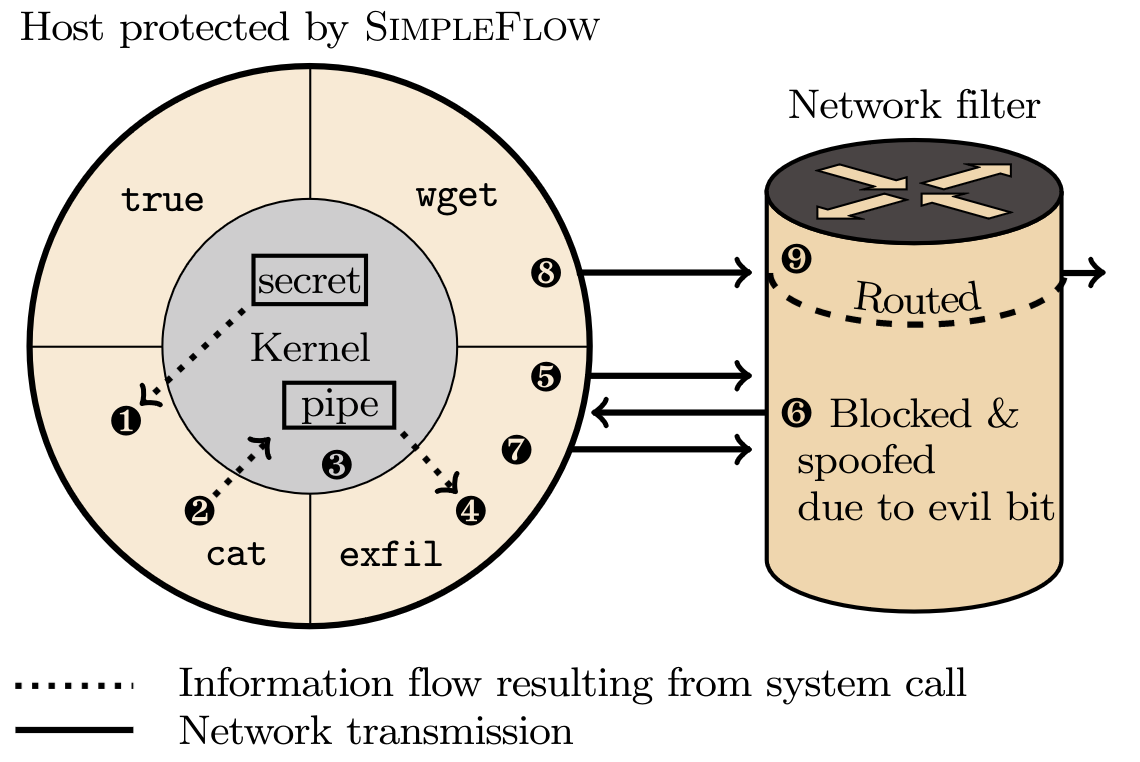
\includegraphics[width=.8\textwidth]{section01/assets/simpleflow_example.png}
    \caption[SimpleFlow Example]{SimpleFlow Being Used to Prevent Exfiltration of Sensitive Data (from \cite{ryan2016})\label{simpleflowexample}}
\end{figure}
\blfootnote{The above numerical SimpleFlow example items were summarized from \cite{ryan2016}.}
\begin{enumerate}[label={\protect\circled{\arabic*}}]
    \item A malicious user uses the \texttt{cat} process to open and read the confidential data in \texttt{secret}.
          Now any further actions processed by this user are tainted by SimpleFlow by being marked with an evil bit 
          and are monitored by the SimpleFlow system.
    \item The malicious user attempts to pipe and exfiltrate the information in \texttt{secret}.
    \item The pipe is forked as a child from the \texttt{cat} process and therefore is also marked as malicious activity by SimpleFlow.
    \item The \texttt{exfil} command reads \texttt{secret} and becomes tainted with the evil bit.
    \item The malicious user attepts to exfiltrate the information from \texttt{secret} to a personal server. 
          The sent packet containing \texttt{secret}'s
          information is marked with an evil bit to be easily recognizable by SimpleFlow as an unsolicited action.
    \item SimpleFlow's network filter notices the malicious user's attempt to exfiltrate the information from \texttt{secret}.
          SimpleFlow sends a fake response to the request to make the malicious user think that the process is being continued.
    \item The malicious user's exfiltration attept on \texttt{secret}'s data is ultimately blocked by SimpleFlow's network filter.
    \item The non-threatening process \texttt{wget} is performed on the system.
    \item SimpleFlow's network filter behaves normally and allows the \texttt{wget} process to continue.
\end{enumerate}


While effective, the research prototype of SimpleFlow is limited in 
that it cannot further specify the security policy of a file beyond 
being confidential and non-confidential \cite{ryan2016}. A resolution 
for SimpleFlow’s issue of a binary security system was therefore sought out and as a solution 
a customized Linux security tool suite was devised. The system would allow the 
privileged user to define hierarchical levels and non-hierarchical 
labels on a system and assign them to both system users and system 
files. This security policy was inspired by the US security 
classification system \cite{natsecinfo} by following the structure of having both levels 
and labels for security. The policy states that both system files and system users may each have one 
security level and zero or more security labels. 

As a running example, pretend that
there is a software company that is working on innovative technology that they want
to be kept secretive so that all files related to the technology are on a need-to-know basis. 
With this proposed security policy, the company could define a system saying which staff have
access to what files. For example, the privileged administrative user who oversees creating the security policy 
could define the hierarchy levels for the company from lowest to highest as
\texttt{public}, \texttt{general\_staff}, \texttt{developer}, \texttt{administrator}, and \texttt{executive\_staff}.
In this example, the company has also split the technology into several projects, 
three of which are named \texttt{alpha}, \texttt{beta}, and \texttt{charlie}. If Alice is an \texttt{administrator} for
both projects \texttt{alpha} and \texttt{beta}, then, with the newly proposed security policy,
she would be given the hierarchical level \texttt{administrator} and the non-hierarchical labels
\texttt{alpha} and \texttt{beta}. 

Continuing the above example, pretend that there is a file to outline how to begin development on project \texttt{alpha} called
\texttt{alpha}\texttt{\_dev}\texttt{\_instructions.txt}. The privileged administrator could assign \texttt{alpha}\texttt{\_dev}\texttt{\_instructions.txt} 
the security level \texttt{developer} and the security label \texttt{alpha}. Alice, who has the security level of \texttt{administrator}
which is placed higher than \texttt{developer} in the level hierarchy 
and who contains the security label \texttt{alpha} can access \texttt{alpha}\texttt{\_dev}\texttt{\_instructions.txt}.
Pretend that there is also a developer in the company named Bob who is a developer for projects \texttt{beta} and \texttt{charlie}. Bob would
have the security level \texttt{developer} which is a proper label to be able to access \texttt{alpha}\texttt{\_dev}\texttt{\_instructions.txt}, but Bob would not
be given the label \texttt{alpha} so therefore would ultimately not have access to \texttt{alpha}\texttt{\_dev}\texttt{\_instructions.txt}.

The newly proposed security policy of levels and labels 
would allow multiple groupings of users such as, in our example, 
more \texttt{developer}s who have access to project \texttt{alpha}, more \texttt{administrator}s that 
have access to multiple projects,
and files that are available to all staff members. With the newly proposed security policy, 
a system administrator would therefore be able 
to flexibly compartmentalize all the files and data that users would have 
access to on a system. Initially, it may seem like other previously-developed access control models may be sufficient
to create a security policy that is ideal for SimpleFlow such as role-based access controls (RBAC).
However, these models are not as ideal as the newly proposed PAMEx secuirty policy.
As stated above, most RBAC simply disallow reading or writing to confidential files on a system, but SimpleFlow 
wants to instead allow that access so as to be able to monitor an attacker's actions. SimpleFlow's primary job is
to record a malicious user's activity on the system and ultimately disallow exfiltrating confidential information
via its network filter. With SimpleFlow having such a particular goal, only a custom security policy such as PAMEx will allow SimpleFlow
to continue to monitor a system the way that it was designed to without interfering with SimpleFlow's actions.
Ideally, the tool suite would be developed as a standalone 
Linux Security Module so as to be tailored to but not mutually 
exclusive for SimpleFlow though. The development of the custom kernel module that would allow the tool suite to be standalone
or ported into SimpleFlow was left to future work.


\subsection{Motivation}
\par 
\vspace{\baselineskip}
\hspace{1em}
In 2022, the author reached out to his advisor, Dr. W. Michael 
Petullo showing interest in the SimpleFlow project and learning more about 
its shortcomings including the binary security policy currently in 
place. Having pursued an emphasis in cybersecurity alongside his 
degree, the author had already had an introduction to Linux security 
but wanted to learn more. The motivation of PAMEx was to aid in and 
further enhance the development of the SimpleFlow project as well as 
to learn more about Linux security at a system level and how it can 
be added to and manipulated. Building a security policy tool system 
from the ground up would give a foundational experience of 
that aspect of security systems. 

Together with his advisor, the author devised and proposed an 
alternative solution for the SimpleFlow security policy than the 
one currently in place. This policy would continue to work on top 
of the LSM interface as SimpleFlow already does and therefore be 
integrated into SimpleFlow easily. The policy’s syntax and 
tools would be user friendly and allow for much greater malleability 
while having a small footprint. Another requirement was to ensure 
that PAMEx's integration would not need to be exclusive 
to SimpleFlow but could be used on many Linux based systems. Developing 
a project of this scale is also a perfect opportunity to research, learn about, and practice the development cycle of 
a project with industry standards.  

}{}\clearpage
\IfFileExists{section04/section}{\section{Introduction}
\newcounter{numitem}

\label{sec:Introduction}
\vspace{\baselineskip}

\subsection{Background}
\par 
\vspace{\baselineskip}
\hspace{1em}
The objective of PAMEx is to work in conjunction with and enhance the 
pre-existing project SimpleFlow, an information-flow-based access 
control system. Even in the modern day, most access control systems 
simply disallow read or write access to confidential files. The 
SimpleFlow project was developed to go beyond most access control 
systems and instead allow malicious users to access confidential 
files up until the point of exfiltration so that SimpleFlow can monitor the user's activity. The way that 
SimpleFlow achieves this is by working on top of the Linux Security 
Module (LSM) interface and rather than simply disallowing read or write 
access like most access control systems do, SimpleFlow instead marks a 
file as either confidential or non-confidential. If a confidential 
file is wrongly accessed, the malicious user’s actions are recorded as they pass 
through the system as information flows. The wrongly accessed 
information is then prevented from being exfiltrated by SimpleFlow's network filter. 
SimpleFlow begins tracking the attacker’s actions as soon as they 
attempt to access the confidential file and therefore can capture the attacker’s 
intentions. This leaves no room for the malicious user to come up with 
a fabricated excuse as to why they were trying to exfiltrate sensitive 
information. As an example of SimpleFlow’s effectiveness, when put to 
practical use during the 2016 Cyber-Defense Exercise, the SimpleFlow 
program proved to perform well with a small overhead. While the 
practical exercise did not make use of all SimpleFlow’s functionality, 
it was able to successfully use SimpleFlow’s network filter which made 
it easy to observe any attempt at exfiltrating data. Within this 
exercise and other testing, SimpleFlow impressed attackers who were 
surprised to find their exfiltration attempts had failed \cite{ryan2016}. 

Figure~\ref{simpleflowexample} was pulled from the paper ``Studying Naive Users and the Insider Threat with SimpleFlow.''
to depict SimpleFlow being used to prevent an exfiltration attempt of sensitive data.
The example starts with a file on the kernel marked as \texttt{secret} which contains sensitive information.

\clearpage

\begin{figure}[h]
    \centering
    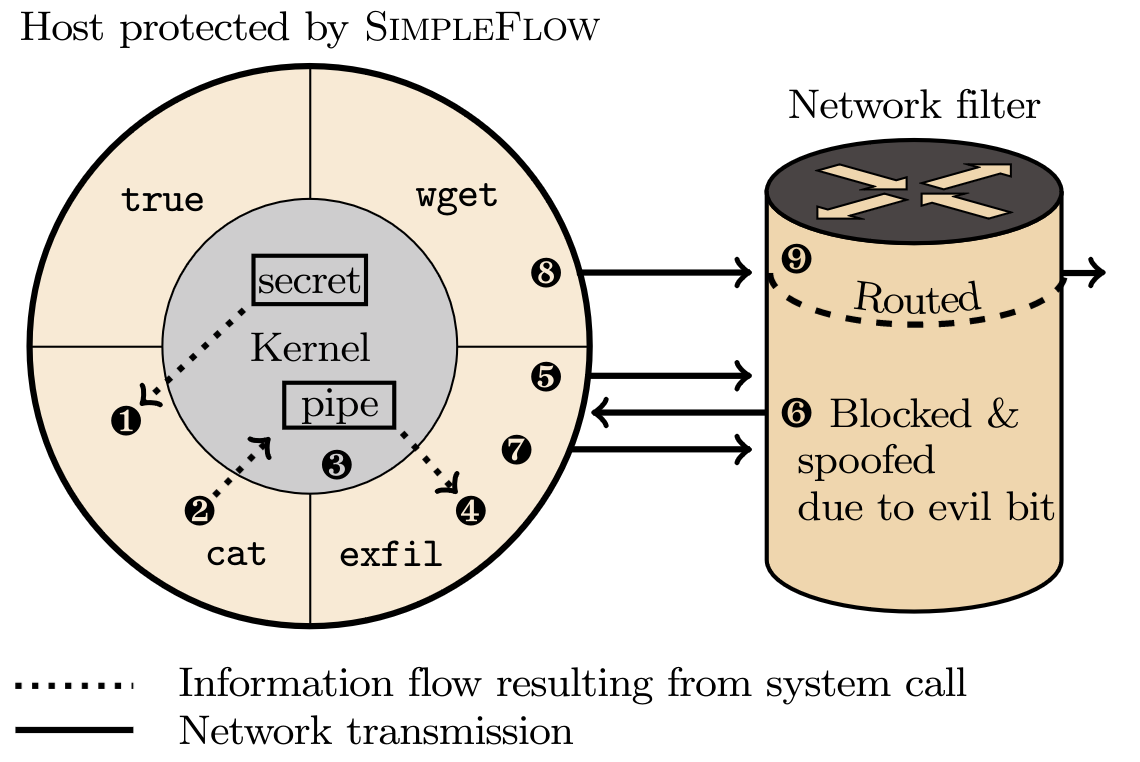
\includegraphics[width=.8\textwidth]{section01/assets/simpleflow_example.png}
    \caption[SimpleFlow Example]{SimpleFlow Being Used to Prevent Exfiltration of Sensitive Data (from \cite{ryan2016})\label{simpleflowexample}}
\end{figure}
\blfootnote{The above numerical SimpleFlow example items were summarized from \cite{ryan2016}.}
\begin{enumerate}[label={\protect\circled{\arabic*}}]
    \item A malicious user uses the \texttt{cat} process to open and read the confidential data in \texttt{secret}.
          Now any further actions processed by this user are tainted by SimpleFlow by being marked with an evil bit 
          and are monitored by the SimpleFlow system.
    \item The malicious user attempts to pipe and exfiltrate the information in \texttt{secret}.
    \item The pipe is forked as a child from the \texttt{cat} process and therefore is also marked as malicious activity by SimpleFlow.
    \item The \texttt{exfil} command reads \texttt{secret} and becomes tainted with the evil bit.
    \item The malicious user attepts to exfiltrate the information from \texttt{secret} to a personal server. 
          The sent packet containing \texttt{secret}'s
          information is marked with an evil bit to be easily recognizable by SimpleFlow as an unsolicited action.
    \item SimpleFlow's network filter notices the malicious user's attempt to exfiltrate the information from \texttt{secret}.
          SimpleFlow sends a fake response to the request to make the malicious user think that the process is being continued.
    \item The malicious user's exfiltration attept on \texttt{secret}'s data is ultimately blocked by SimpleFlow's network filter.
    \item The non-threatening process \texttt{wget} is performed on the system.
    \item SimpleFlow's network filter behaves normally and allows the \texttt{wget} process to continue.
\end{enumerate}


While effective, the research prototype of SimpleFlow is limited in 
that it cannot further specify the security policy of a file beyond 
being confidential and non-confidential \cite{ryan2016}. A resolution 
for SimpleFlow’s issue of a binary security system was therefore sought out and as a solution 
a customized Linux security tool suite was devised. The system would allow the 
privileged user to define hierarchical levels and non-hierarchical 
labels on a system and assign them to both system users and system 
files. This security policy was inspired by the US security 
classification system \cite{natsecinfo} by following the structure of having both levels 
and labels for security. The policy states that both system files and system users may each have one 
security level and zero or more security labels. 

As a running example, pretend that
there is a software company that is working on innovative technology that they want
to be kept secretive so that all files related to the technology are on a need-to-know basis. 
With this proposed security policy, the company could define a system saying which staff have
access to what files. For example, the privileged administrative user who oversees creating the security policy 
could define the hierarchy levels for the company from lowest to highest as
\texttt{public}, \texttt{general\_staff}, \texttt{developer}, \texttt{administrator}, and \texttt{executive\_staff}.
In this example, the company has also split the technology into several projects, 
three of which are named \texttt{alpha}, \texttt{beta}, and \texttt{charlie}. If Alice is an \texttt{administrator} for
both projects \texttt{alpha} and \texttt{beta}, then, with the newly proposed security policy,
she would be given the hierarchical level \texttt{administrator} and the non-hierarchical labels
\texttt{alpha} and \texttt{beta}. 

Continuing the above example, pretend that there is a file to outline how to begin development on project \texttt{alpha} called
\texttt{alpha}\texttt{\_dev}\texttt{\_instructions.txt}. The privileged administrator could assign \texttt{alpha}\texttt{\_dev}\texttt{\_instructions.txt} 
the security level \texttt{developer} and the security label \texttt{alpha}. Alice, who has the security level of \texttt{administrator}
which is placed higher than \texttt{developer} in the level hierarchy 
and who contains the security label \texttt{alpha} can access \texttt{alpha}\texttt{\_dev}\texttt{\_instructions.txt}.
Pretend that there is also a developer in the company named Bob who is a developer for projects \texttt{beta} and \texttt{charlie}. Bob would
have the security level \texttt{developer} which is a proper label to be able to access \texttt{alpha}\texttt{\_dev}\texttt{\_instructions.txt}, but Bob would not
be given the label \texttt{alpha} so therefore would ultimately not have access to \texttt{alpha}\texttt{\_dev}\texttt{\_instructions.txt}.

The newly proposed security policy of levels and labels 
would allow multiple groupings of users such as, in our example, 
more \texttt{developer}s who have access to project \texttt{alpha}, more \texttt{administrator}s that 
have access to multiple projects,
and files that are available to all staff members. With the newly proposed security policy, 
a system administrator would therefore be able 
to flexibly compartmentalize all the files and data that users would have 
access to on a system. Initially, it may seem like other previously-developed access control models may be sufficient
to create a security policy that is ideal for SimpleFlow such as role-based access controls (RBAC).
However, these models are not as ideal as the newly proposed PAMEx secuirty policy.
As stated above, most RBAC simply disallow reading or writing to confidential files on a system, but SimpleFlow 
wants to instead allow that access so as to be able to monitor an attacker's actions. SimpleFlow's primary job is
to record a malicious user's activity on the system and ultimately disallow exfiltrating confidential information
via its network filter. With SimpleFlow having such a particular goal, only a custom security policy such as PAMEx will allow SimpleFlow
to continue to monitor a system the way that it was designed to without interfering with SimpleFlow's actions.
Ideally, the tool suite would be developed as a standalone 
Linux Security Module so as to be tailored to but not mutually 
exclusive for SimpleFlow though. The development of the custom kernel module that would allow the tool suite to be standalone
or ported into SimpleFlow was left to future work.


\subsection{Motivation}
\par 
\vspace{\baselineskip}
\hspace{1em}
In 2022, the author reached out to his advisor, Dr. W. Michael 
Petullo showing interest in the SimpleFlow project and learning more about 
its shortcomings including the binary security policy currently in 
place. Having pursued an emphasis in cybersecurity alongside his 
degree, the author had already had an introduction to Linux security 
but wanted to learn more. The motivation of PAMEx was to aid in and 
further enhance the development of the SimpleFlow project as well as 
to learn more about Linux security at a system level and how it can 
be added to and manipulated. Building a security policy tool system 
from the ground up would give a foundational experience of 
that aspect of security systems. 

Together with his advisor, the author devised and proposed an 
alternative solution for the SimpleFlow security policy than the 
one currently in place. This policy would continue to work on top 
of the LSM interface as SimpleFlow already does and therefore be 
integrated into SimpleFlow easily. The policy’s syntax and 
tools would be user friendly and allow for much greater malleability 
while having a small footprint. Another requirement was to ensure 
that PAMEx's integration would not need to be exclusive 
to SimpleFlow but could be used on many Linux based systems. Developing 
a project of this scale is also a perfect opportunity to research, learn about, and practice the development cycle of 
a project with industry standards.  

}{}\clearpage
\IfFileExists{section04/section}{\section{Introduction}
\newcounter{numitem}

\label{sec:Introduction}
\vspace{\baselineskip}

\subsection{Background}
\par 
\vspace{\baselineskip}
\hspace{1em}
The objective of PAMEx is to work in conjunction with and enhance the 
pre-existing project SimpleFlow, an information-flow-based access 
control system. Even in the modern day, most access control systems 
simply disallow read or write access to confidential files. The 
SimpleFlow project was developed to go beyond most access control 
systems and instead allow malicious users to access confidential 
files up until the point of exfiltration so that SimpleFlow can monitor the user's activity. The way that 
SimpleFlow achieves this is by working on top of the Linux Security 
Module (LSM) interface and rather than simply disallowing read or write 
access like most access control systems do, SimpleFlow instead marks a 
file as either confidential or non-confidential. If a confidential 
file is wrongly accessed, the malicious user’s actions are recorded as they pass 
through the system as information flows. The wrongly accessed 
information is then prevented from being exfiltrated by SimpleFlow's network filter. 
SimpleFlow begins tracking the attacker’s actions as soon as they 
attempt to access the confidential file and therefore can capture the attacker’s 
intentions. This leaves no room for the malicious user to come up with 
a fabricated excuse as to why they were trying to exfiltrate sensitive 
information. As an example of SimpleFlow’s effectiveness, when put to 
practical use during the 2016 Cyber-Defense Exercise, the SimpleFlow 
program proved to perform well with a small overhead. While the 
practical exercise did not make use of all SimpleFlow’s functionality, 
it was able to successfully use SimpleFlow’s network filter which made 
it easy to observe any attempt at exfiltrating data. Within this 
exercise and other testing, SimpleFlow impressed attackers who were 
surprised to find their exfiltration attempts had failed \cite{ryan2016}. 

Figure~\ref{simpleflowexample} was pulled from the paper ``Studying Naive Users and the Insider Threat with SimpleFlow.''
to depict SimpleFlow being used to prevent an exfiltration attempt of sensitive data.
The example starts with a file on the kernel marked as \texttt{secret} which contains sensitive information.

\clearpage

\begin{figure}[h]
    \centering
    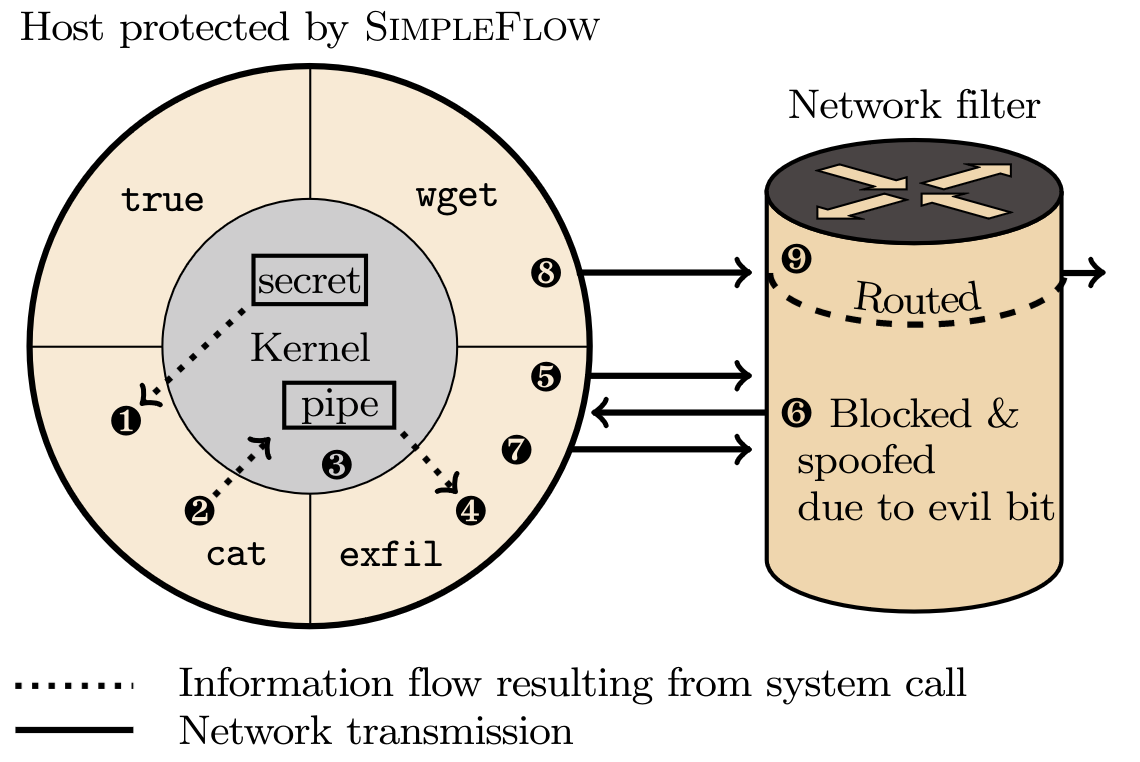
\includegraphics[width=.8\textwidth]{section01/assets/simpleflow_example.png}
    \caption[SimpleFlow Example]{SimpleFlow Being Used to Prevent Exfiltration of Sensitive Data (from \cite{ryan2016})\label{simpleflowexample}}
\end{figure}
\blfootnote{The above numerical SimpleFlow example items were summarized from \cite{ryan2016}.}
\begin{enumerate}[label={\protect\circled{\arabic*}}]
    \item A malicious user uses the \texttt{cat} process to open and read the confidential data in \texttt{secret}.
          Now any further actions processed by this user are tainted by SimpleFlow by being marked with an evil bit 
          and are monitored by the SimpleFlow system.
    \item The malicious user attempts to pipe and exfiltrate the information in \texttt{secret}.
    \item The pipe is forked as a child from the \texttt{cat} process and therefore is also marked as malicious activity by SimpleFlow.
    \item The \texttt{exfil} command reads \texttt{secret} and becomes tainted with the evil bit.
    \item The malicious user attepts to exfiltrate the information from \texttt{secret} to a personal server. 
          The sent packet containing \texttt{secret}'s
          information is marked with an evil bit to be easily recognizable by SimpleFlow as an unsolicited action.
    \item SimpleFlow's network filter notices the malicious user's attempt to exfiltrate the information from \texttt{secret}.
          SimpleFlow sends a fake response to the request to make the malicious user think that the process is being continued.
    \item The malicious user's exfiltration attept on \texttt{secret}'s data is ultimately blocked by SimpleFlow's network filter.
    \item The non-threatening process \texttt{wget} is performed on the system.
    \item SimpleFlow's network filter behaves normally and allows the \texttt{wget} process to continue.
\end{enumerate}


While effective, the research prototype of SimpleFlow is limited in 
that it cannot further specify the security policy of a file beyond 
being confidential and non-confidential \cite{ryan2016}. A resolution 
for SimpleFlow’s issue of a binary security system was therefore sought out and as a solution 
a customized Linux security tool suite was devised. The system would allow the 
privileged user to define hierarchical levels and non-hierarchical 
labels on a system and assign them to both system users and system 
files. This security policy was inspired by the US security 
classification system \cite{natsecinfo} by following the structure of having both levels 
and labels for security. The policy states that both system files and system users may each have one 
security level and zero or more security labels. 

As a running example, pretend that
there is a software company that is working on innovative technology that they want
to be kept secretive so that all files related to the technology are on a need-to-know basis. 
With this proposed security policy, the company could define a system saying which staff have
access to what files. For example, the privileged administrative user who oversees creating the security policy 
could define the hierarchy levels for the company from lowest to highest as
\texttt{public}, \texttt{general\_staff}, \texttt{developer}, \texttt{administrator}, and \texttt{executive\_staff}.
In this example, the company has also split the technology into several projects, 
three of which are named \texttt{alpha}, \texttt{beta}, and \texttt{charlie}. If Alice is an \texttt{administrator} for
both projects \texttt{alpha} and \texttt{beta}, then, with the newly proposed security policy,
she would be given the hierarchical level \texttt{administrator} and the non-hierarchical labels
\texttt{alpha} and \texttt{beta}. 

Continuing the above example, pretend that there is a file to outline how to begin development on project \texttt{alpha} called
\texttt{alpha}\texttt{\_dev}\texttt{\_instructions.txt}. The privileged administrator could assign \texttt{alpha}\texttt{\_dev}\texttt{\_instructions.txt} 
the security level \texttt{developer} and the security label \texttt{alpha}. Alice, who has the security level of \texttt{administrator}
which is placed higher than \texttt{developer} in the level hierarchy 
and who contains the security label \texttt{alpha} can access \texttt{alpha}\texttt{\_dev}\texttt{\_instructions.txt}.
Pretend that there is also a developer in the company named Bob who is a developer for projects \texttt{beta} and \texttt{charlie}. Bob would
have the security level \texttt{developer} which is a proper label to be able to access \texttt{alpha}\texttt{\_dev}\texttt{\_instructions.txt}, but Bob would not
be given the label \texttt{alpha} so therefore would ultimately not have access to \texttt{alpha}\texttt{\_dev}\texttt{\_instructions.txt}.

The newly proposed security policy of levels and labels 
would allow multiple groupings of users such as, in our example, 
more \texttt{developer}s who have access to project \texttt{alpha}, more \texttt{administrator}s that 
have access to multiple projects,
and files that are available to all staff members. With the newly proposed security policy, 
a system administrator would therefore be able 
to flexibly compartmentalize all the files and data that users would have 
access to on a system. Initially, it may seem like other previously-developed access control models may be sufficient
to create a security policy that is ideal for SimpleFlow such as role-based access controls (RBAC).
However, these models are not as ideal as the newly proposed PAMEx secuirty policy.
As stated above, most RBAC simply disallow reading or writing to confidential files on a system, but SimpleFlow 
wants to instead allow that access so as to be able to monitor an attacker's actions. SimpleFlow's primary job is
to record a malicious user's activity on the system and ultimately disallow exfiltrating confidential information
via its network filter. With SimpleFlow having such a particular goal, only a custom security policy such as PAMEx will allow SimpleFlow
to continue to monitor a system the way that it was designed to without interfering with SimpleFlow's actions.
Ideally, the tool suite would be developed as a standalone 
Linux Security Module so as to be tailored to but not mutually 
exclusive for SimpleFlow though. The development of the custom kernel module that would allow the tool suite to be standalone
or ported into SimpleFlow was left to future work.


\subsection{Motivation}
\par 
\vspace{\baselineskip}
\hspace{1em}
In 2022, the author reached out to his advisor, Dr. W. Michael 
Petullo showing interest in the SimpleFlow project and learning more about 
its shortcomings including the binary security policy currently in 
place. Having pursued an emphasis in cybersecurity alongside his 
degree, the author had already had an introduction to Linux security 
but wanted to learn more. The motivation of PAMEx was to aid in and 
further enhance the development of the SimpleFlow project as well as 
to learn more about Linux security at a system level and how it can 
be added to and manipulated. Building a security policy tool system 
from the ground up would give a foundational experience of 
that aspect of security systems. 

Together with his advisor, the author devised and proposed an 
alternative solution for the SimpleFlow security policy than the 
one currently in place. This policy would continue to work on top 
of the LSM interface as SimpleFlow already does and therefore be 
integrated into SimpleFlow easily. The policy’s syntax and 
tools would be user friendly and allow for much greater malleability 
while having a small footprint. Another requirement was to ensure 
that PAMEx's integration would not need to be exclusive 
to SimpleFlow but could be used on many Linux based systems. Developing 
a project of this scale is also a perfect opportunity to research, learn about, and practice the development cycle of 
a project with industry standards.  

}{}\clearpage

%% BIBLIOGRAPHY
% \section*{Bibliography}
\begin{thebibliography}{14}
    \addcontentsline{toc}{section}{Bibliography}

\bibitem{jorgensen2021}
Jorgensen, Paul C. \textit{Software Testing: A Craftsmans Approach}. Auerbach Publications, 2021.

\bibitem{kung2014}
Kung, David C. \textit{Object-Oriented Software Engineering: An Agile Unified Methodology}. McGraw-Hill, 2014.

\bibitem{lauber}
Pluggable Authentication Modules (PAM), https://www.redhat.com/sysadmin/pluggable-authentication-modules-pam, last accessed 15 April 2023.

\bibitem{lacey2015}
Lacey, Mitch. \textit{The Scrum Field Guide: Practical Advice For Your First Year}. Addison-Wesley, 2015.

\bibitem{levine2009}
Levine, John. \textit{Flex \& Bison}. O'Reilly, 2009.

\bibitem{levine1995}
Levine, John R., et al. \textit{Lex \& Yacc}. O'Reilly, 1995.

\bibitem{kerneldocs}
The Linux Kernel Documentation, https://www.kernel.org/doc/html/latest/, last accessed 15 April 2023.

\bibitem{linuxpam}
Linux-Pam/Linux-Pam: Linux PAM (Pluggable Authentication Modules for Linux) Project, https://github.com/linux-pam/linux-pam, last accessed 15 April 2023.

\bibitem{man7pam}
Linux-PAM, ``pam - Pluggable Authentication Modules for Linux'', Linux-PAM Manual, Release 1.3.1, 2020.

\bibitem{natsecinfo}
Senate Select Committee on Intelligence. ``National Security Information'' Senate Select Committee on Intelligence, https://www.intelligence.senate.gov/laws/national-security-information

\bibitem{ryan2016}
Ryan Johnson, Jessie Lass, W. Michael Petullo. ``Studying Naive Users and the Insider Threat with SimpleFlow'' Proceedings of the 8th ACM CCS International Workshop on Managing Insider Security Threats, 2016.

\bibitem{scrumorg}
What is Scrum?, https://www.scrum.org/learning-series/what-is-scrum, last accessed 15 April 2023.

\bibitem{selinux}
SELinux Project, https://selinuxproject.org/, last accessed 15 April 2023.

\bibitem{man7xattr}
T. Ts'o, ``xattr - Extended attributes,'' Linux Programmer's Manual, xattr(7), 2021.

\end{thebibliography}

\clearpage

% %%% APPENDICES
% \section{Appendices}
% \label{sec:appendices}
% \clearpage

\end{document}
